
\section{Bedienoberfläche}

\newcounter{gui}\setcounter{gui}{10}

\begin{description}[leftmargin=5em, style=sameline]	
	\begin{lhp}{gui}{GUI}{gui:vorraum}
		\item[Name:] Anmeldung
		\item[Beschreibung:] Interface für Anmeldung
		\item[Relevante Systemfunktionen:] \ref{funk:zugriff}
		\item[Abbildungen:] \ref{gui:anm}
	\end{lhp}
\end{description}

\begin{description}[leftmargin=5em, style=sameline]	
	\begin{lhp}{gui}{GUI}{gui:reg}
		\item[Name:] Registrierung
		\item[Beschreibung:] Interface zum Registrieren
		\item[Relevante Systemfunktionen:] \ref{funk:zugriff}
		\item[Abbildungen:] \ref{gui:reg}
	\end{lhp}
\end{description}

\begin{description}[leftmargin=5em, style=sameline]	
	\begin{lhp}{gui}{GUI}{gui:lobby}
		\item[Name:] Lobby
		\item[Beschreibung:] Ansicht der Lobby
		\item[Relevante Systemfunktionen:] \ref{funk:spielraum}
		\item[Abbildungen:] \ref{gui:lob}
	\end{lhp}
\end{description}

\begin{description}[leftmargin=5em, style=sameline]	
	\begin{lhp}{gui}{GUI}{gui:spielerst}
		\item[Name:] Spielraum erstellen
		\item[Beschreibung:] Ansicht, um einen Spielraum zu erstellen.
		\item[Relevante Systemfunktionen:] \ref{funk:spielraum}
		\item[Abbildungen:] \ref{gui:spielerst}
	\end{lhp}
\end{description}

\begin{description}[leftmargin=5em, style=sameline]	
	\begin{lhp}{gui}{GUI}{gui:spielr}
		\item[Name:] Spielraum
		\item[Beschreibung:] Ansicht auf einen Spielraum.
		\item[Relevante Systemfunktionen:] \ref{funk:spielraum}
		\item[Abbildungen:] \ref{gui:spielr}
	\end{lhp}
\end{description}

\begin{description}[leftmargin=5em, style=sameline]	
	\begin{lhp}{gui}{GUI}{gui:spiel}
		\item[Name:] Spielübersicht
		\item[Beschreibung:] Ansicht auf das Spielfeld.
		\item[Relevante Systemfunktionen:] \ref{funk:spielverw}
		\item[Abbildungen:] \ref{gui:spiel}
	\end{lhp}
\end{description}

\begin{description}[leftmargin=5em, style=sameline]	
	\begin{lhp}{gui}{GUI}{gui:handel}
		\item[Name:] Handelfenster
		\item[Beschreibung:] Ansicht des Handelfensters.
		\item[Relevante Systemfunktionen:] \ref{funk:spielverw}
		\item[Abbildungen:] \ref{gui:handel}
	\end{lhp}
\end{description}

\begin{description}[leftmargin=5em, style=sameline]	
	\begin{lhp}{gui}{GUI}{gui:gew}
		\item[Name:] Gewinnerübersicht
		\item[Beschreibung:] Übersicht des Spielergebnisses.
		\item[Relevante Systemfunktionen:] \ref{funk:spielverw}
		\item[Abbildungen:] \ref{gui:gew}
	\end{lhp}
\end{description}

\begin{description}[leftmargin=5em, style=sameline]	
	\begin{lhp}{gui}{GUI}{gui:uebersicht}
		\item[Name:] Gesamtübersicht
		\item[Beschreibung:] Übersicht über alle Spielfenster.
		\item[Relevante Systemfunktionen:] \ref{funk:spielverw}
		\item[Abbildungen:] \ref{gui:uebersicht}
	\end{lhp}
\end{description}


\begin{figure}
	\centering
	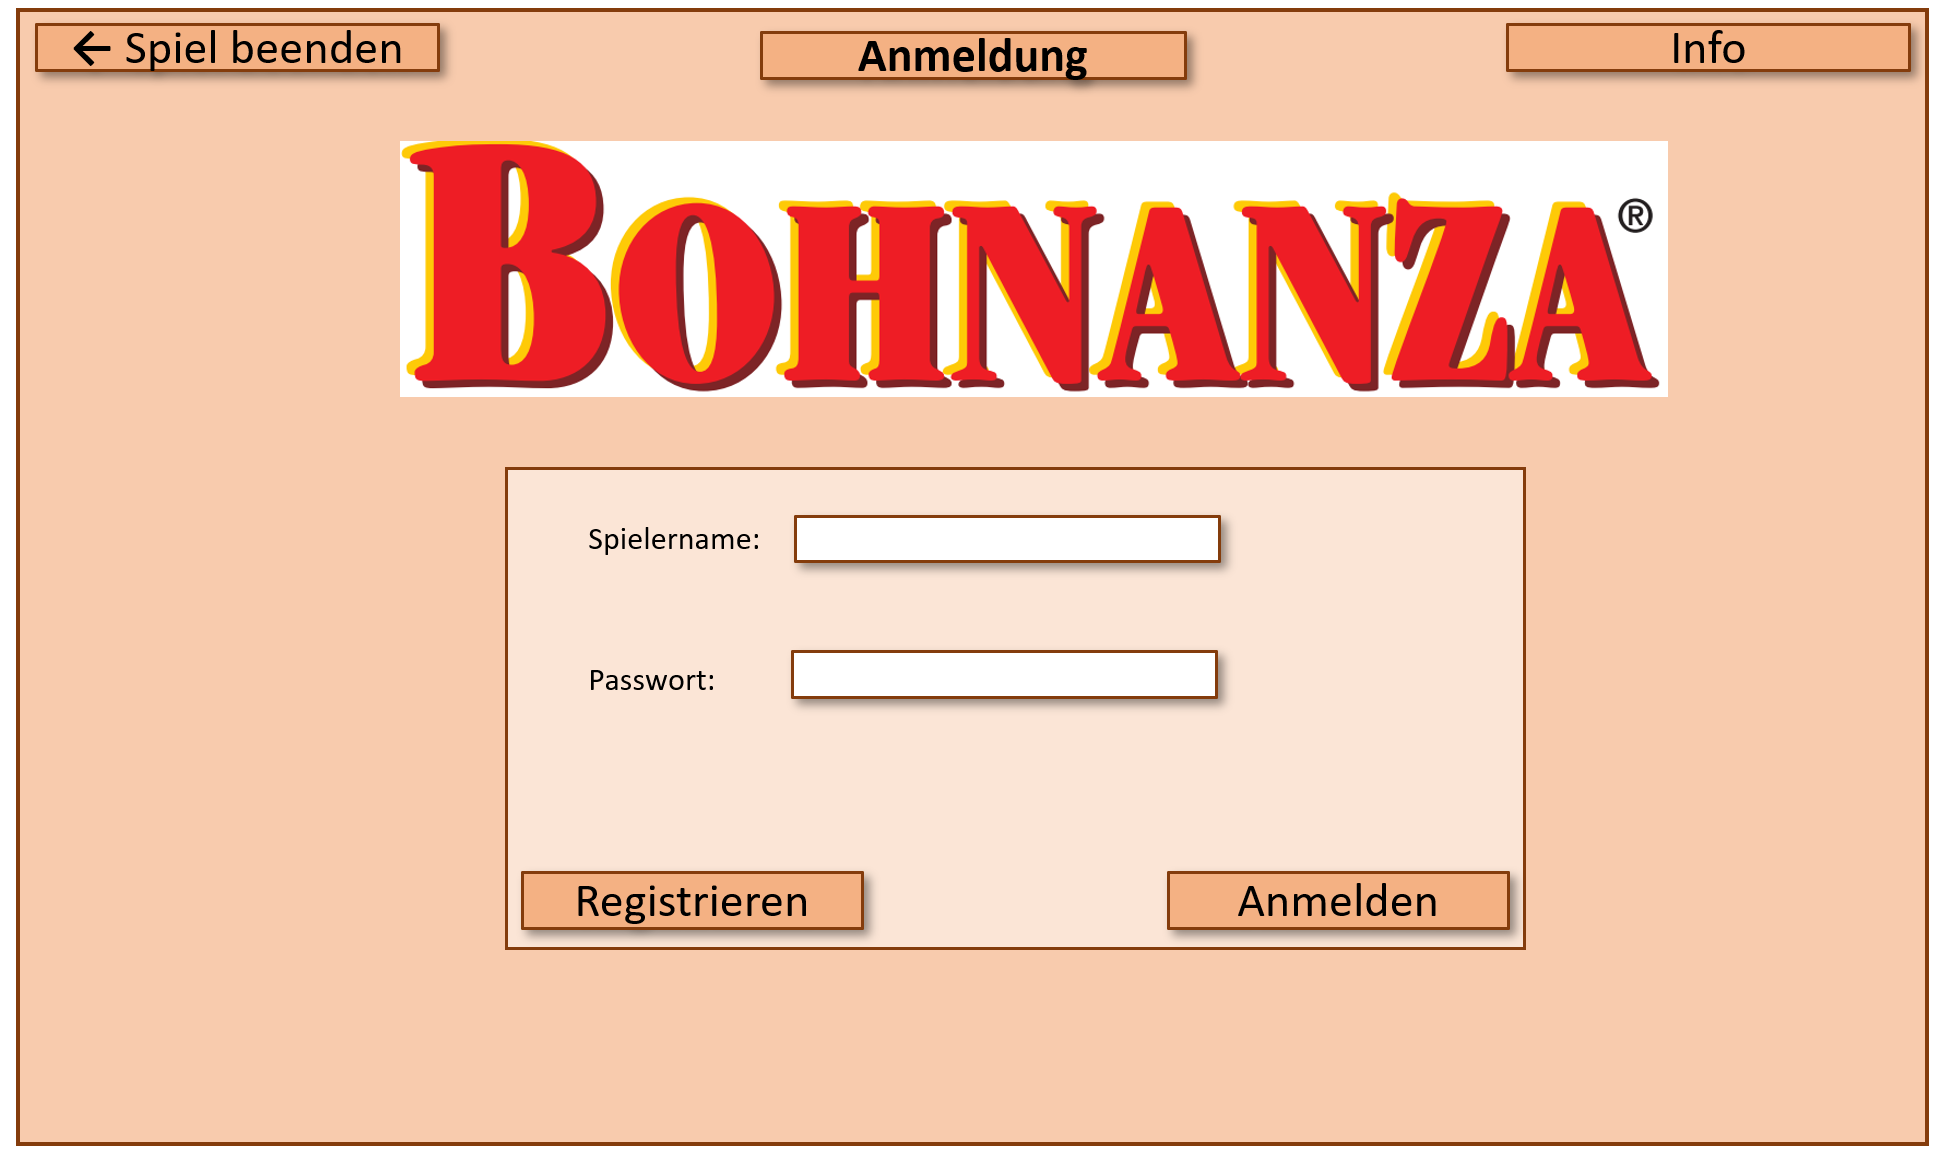
\includegraphics{img/anm}
	\caption{Fenster zur Anmeldung}
	\label{gui:anm}
\end{figure}

\begin{figure}
	\centering
	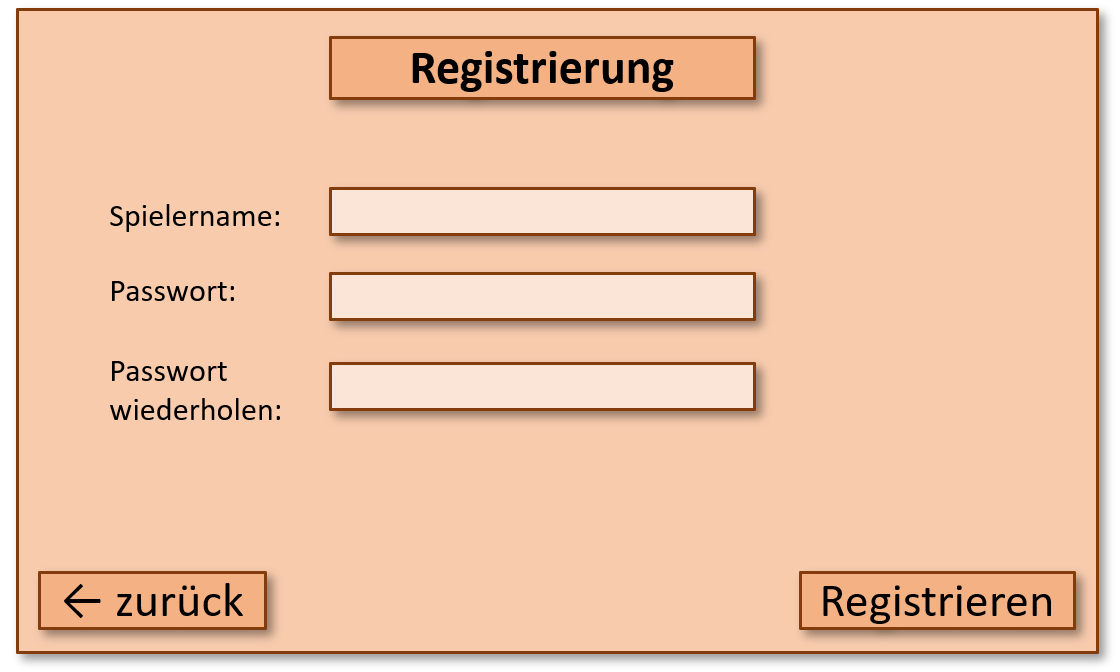
\includegraphics{img/reg}
	\caption{Fenster zum Registrieren}
	\label{gui:reg}
\end{figure}

\begin{figure}
	\centering
	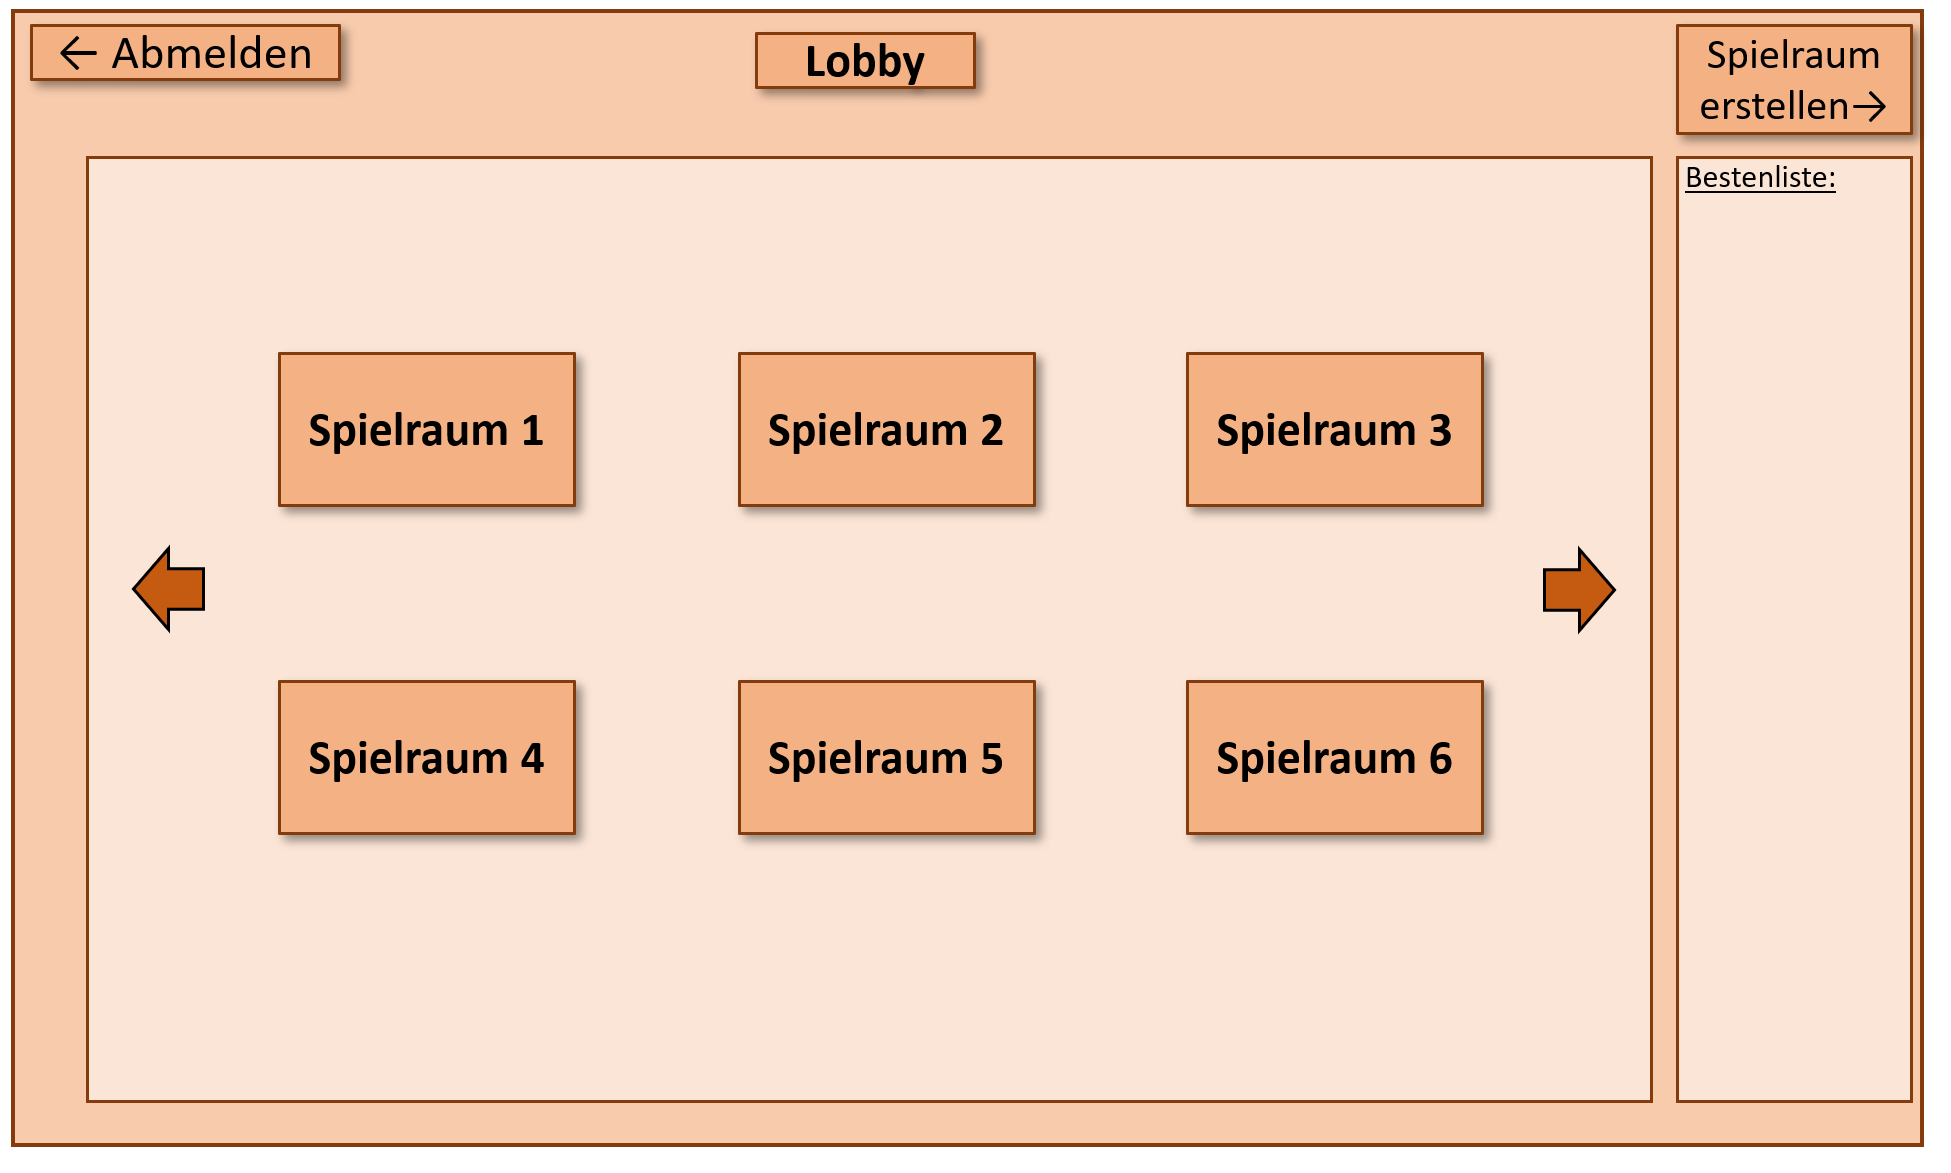
\includegraphics{img/lob}
	\caption{Ansicht der Lobby}
	\label{gui:lob}
\end{figure}

\begin{figure}
	\centering
	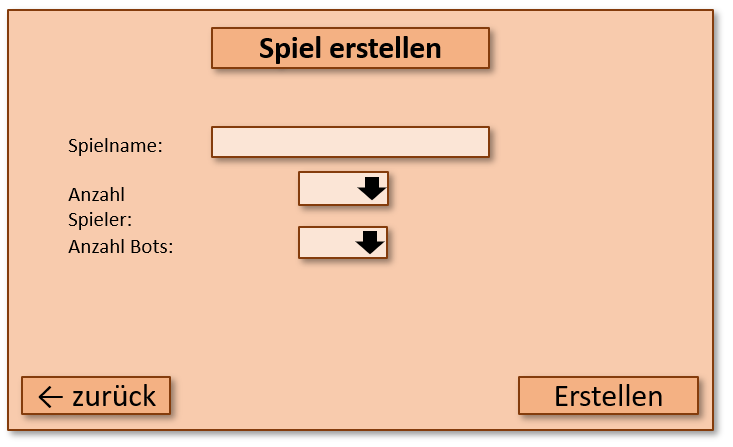
\includegraphics{img/spielerst}
	\caption{Fenster zum Spielerstellen}
	\label{gui:spielerst}
\end{figure}

\begin{figure}
	\centering
	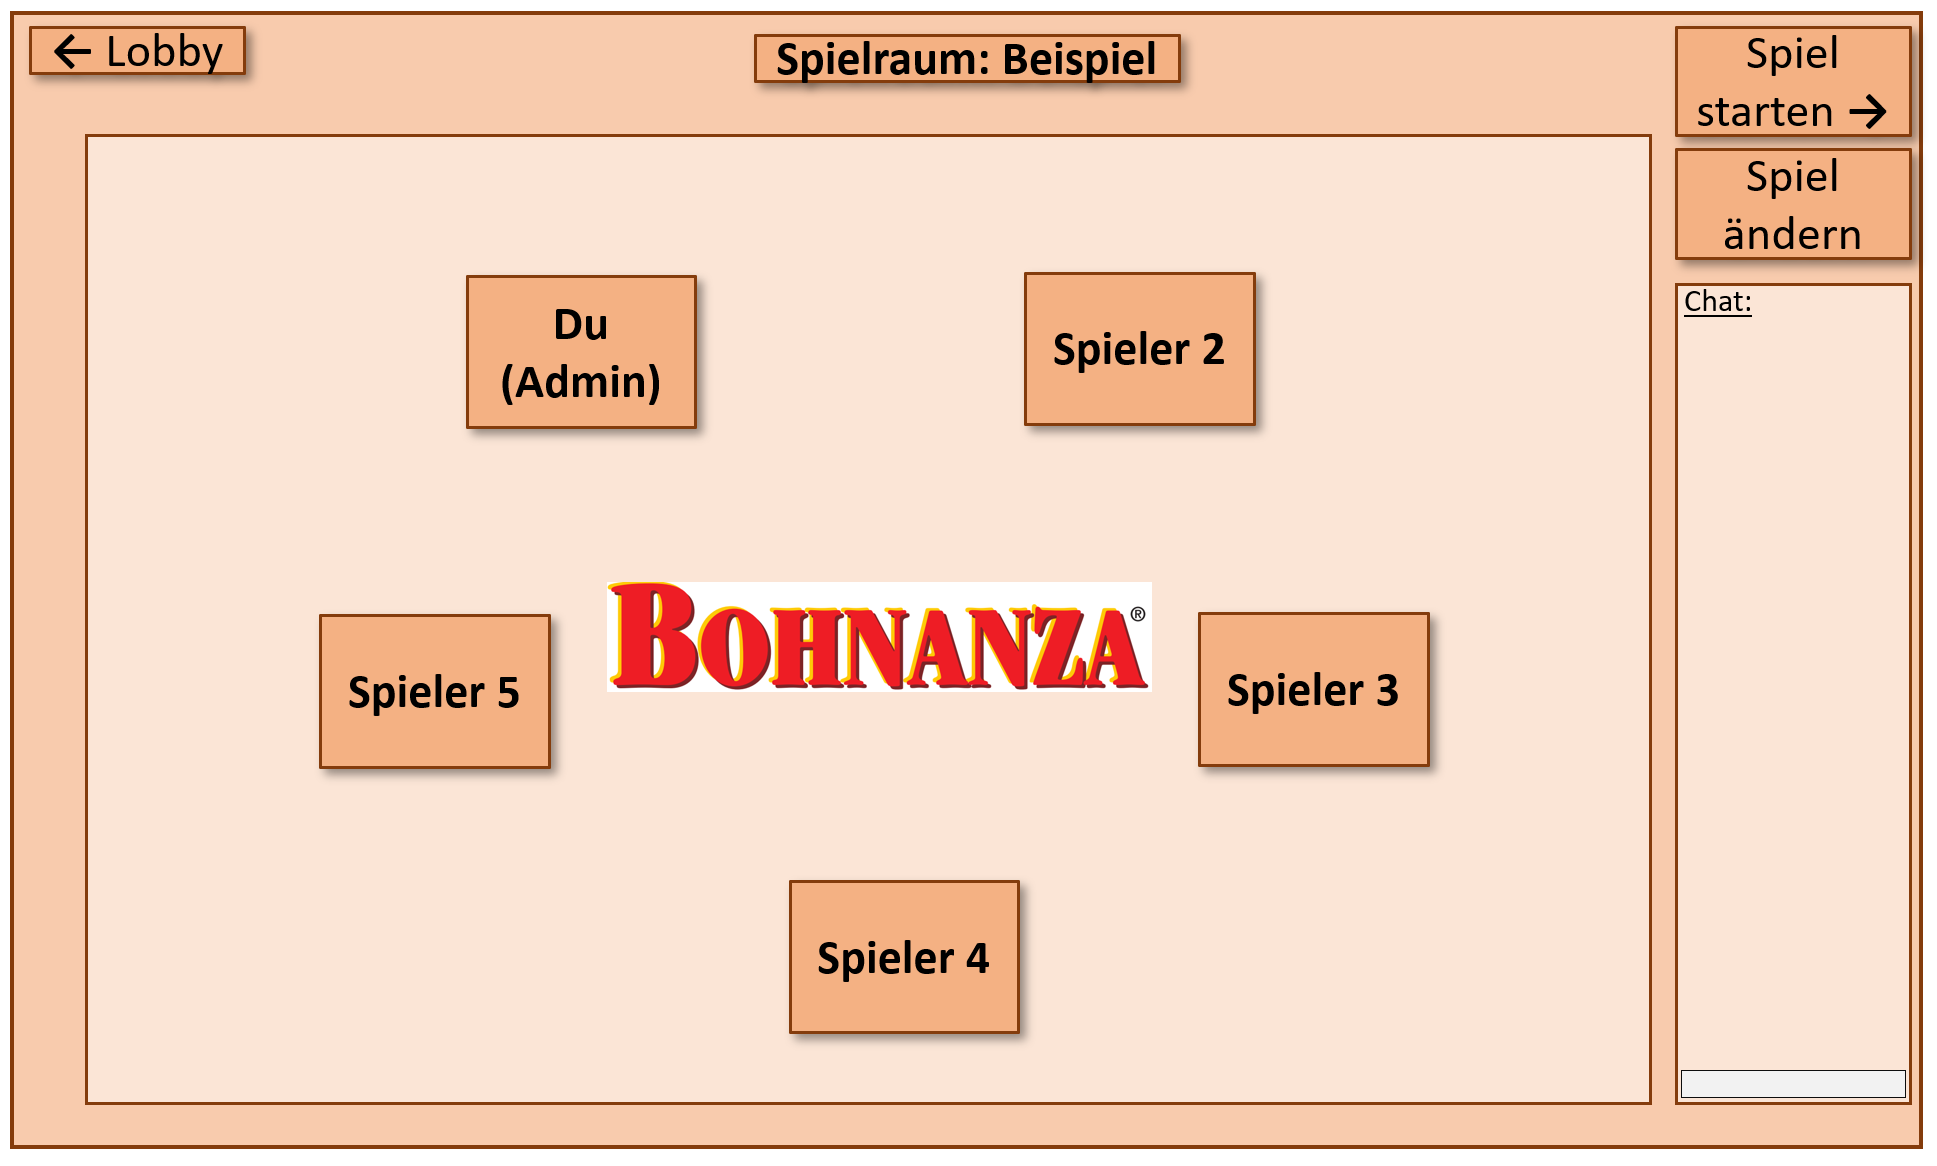
\includegraphics{img/spielr}
	\caption{Ansicht auf einen Spielraum}
	\label{gui:spielr}
\end{figure}

\begin{figure}
	\centering
	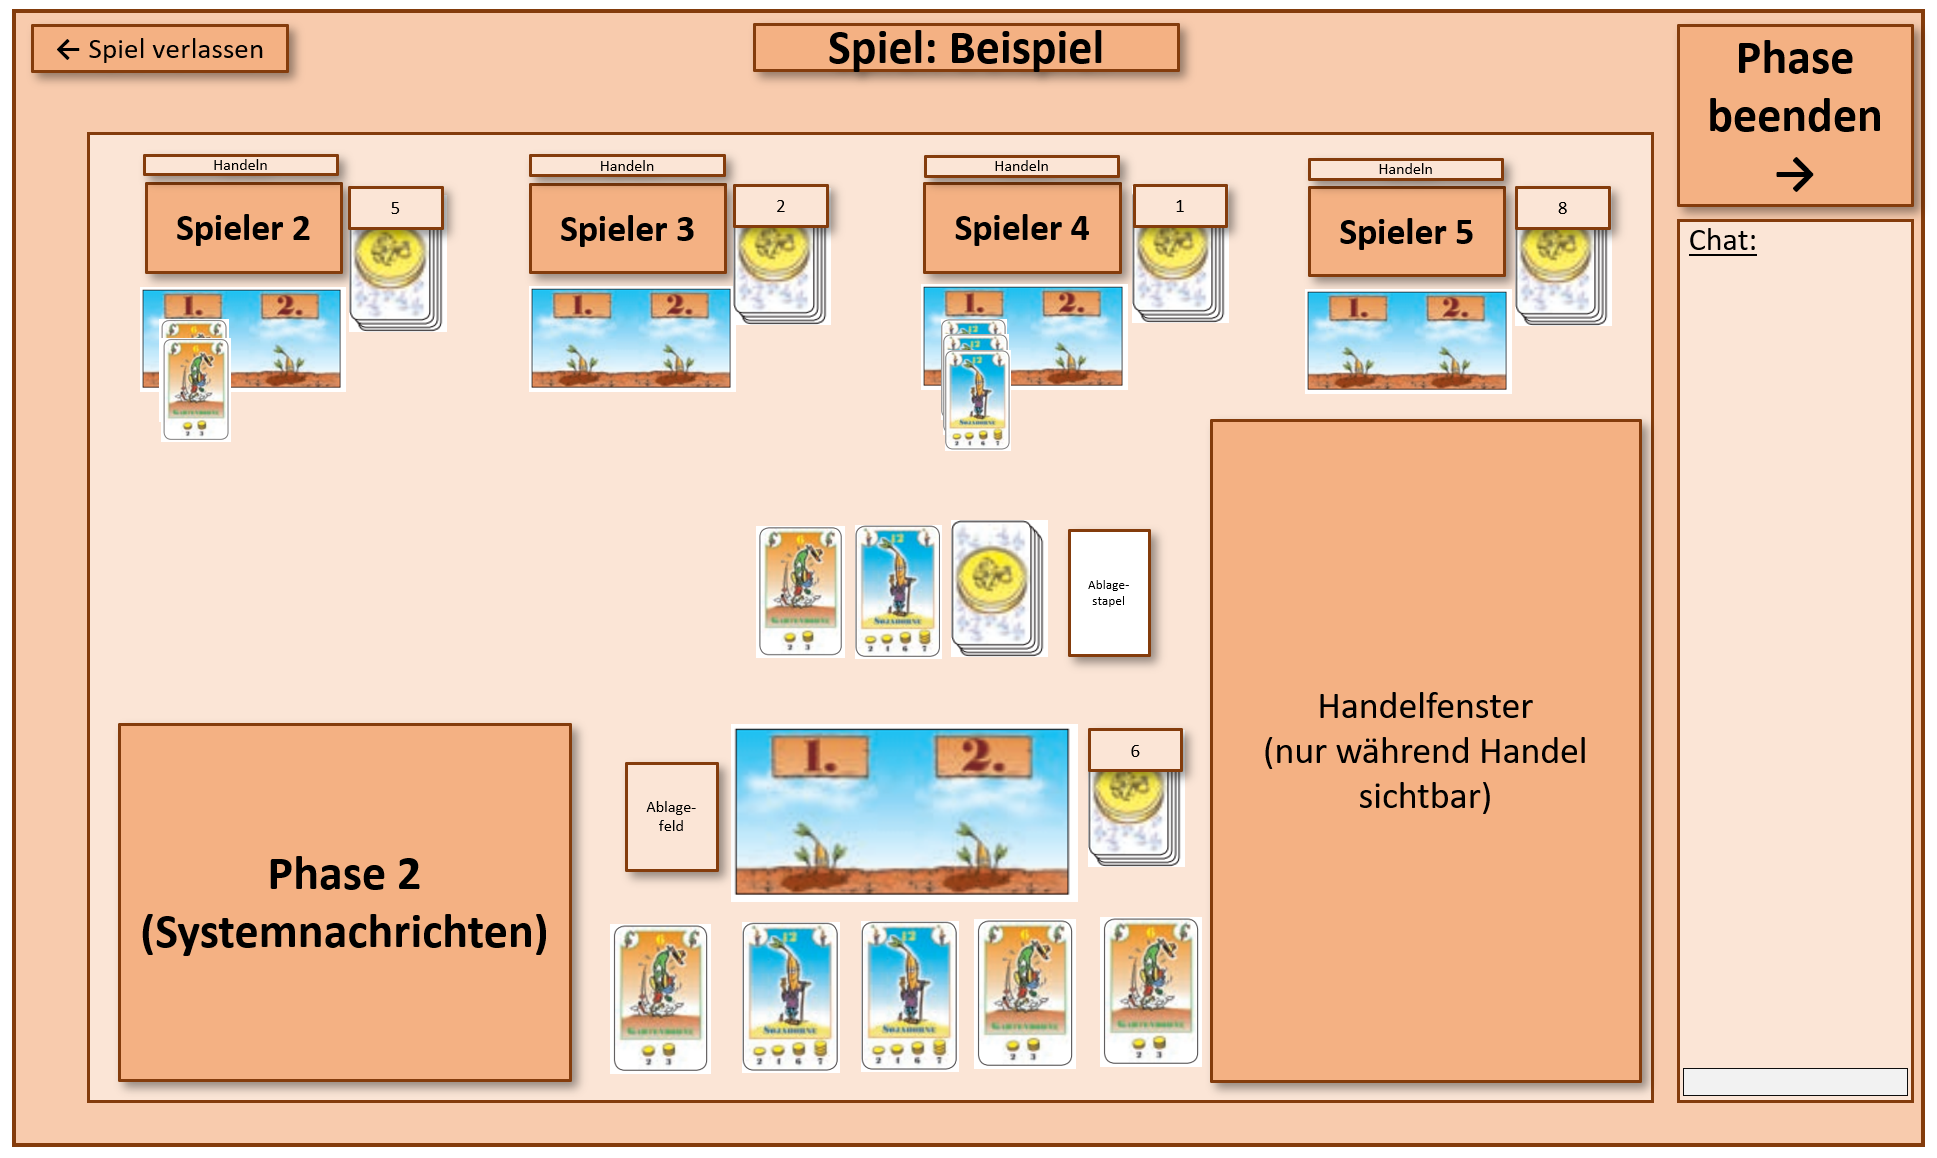
\includegraphics{img/spiel}
	\caption{Ansicht auf das Spielfeld}
	\label{gui:spiel}
\end{figure}

\begin{figure}
	\centering
	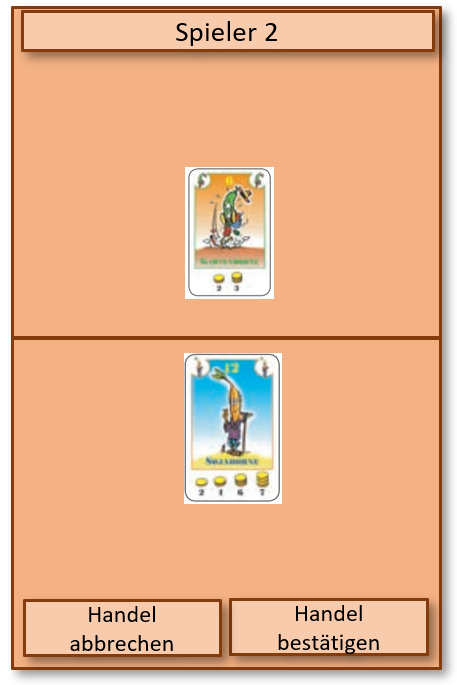
\includegraphics{img/handel}
	\caption{Ansicht des Handelfensters}
	\label{gui:handel}
\end{figure}

\begin{figure}
	\centering
	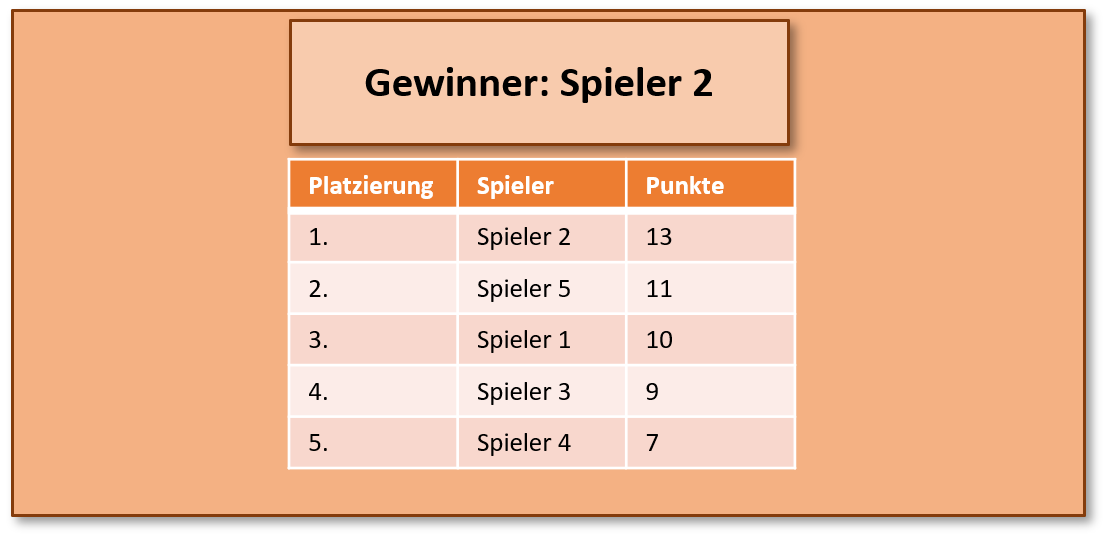
\includegraphics{img/gew}
	\caption{Ansicht des Gewinnerfensters}
	\label{gui:gew}
\end{figure}

\begin{figure}
	\centering
	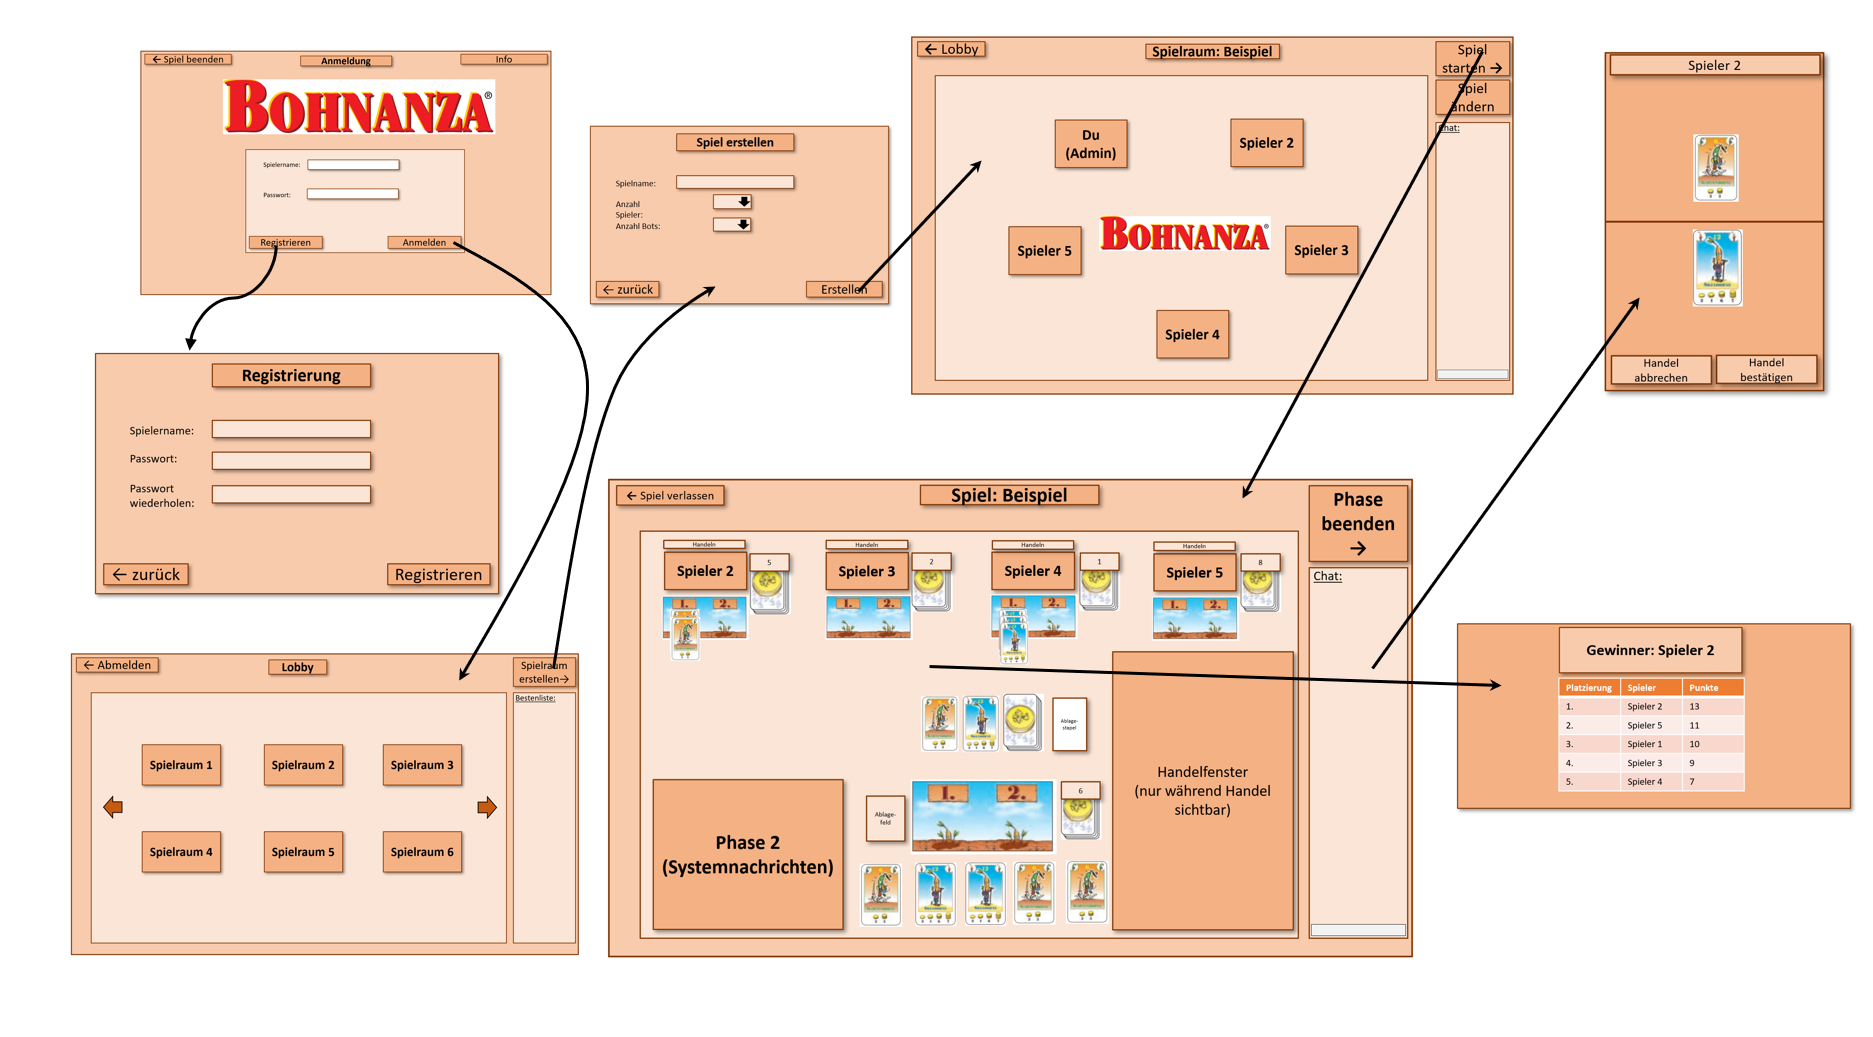
\includegraphics{img/uebersicht}
	\caption{Übersicht über alle Spielfenster}
	\label{gui:uebersicht}
\end{figure}